\chapter{弱い場、重力波、そして作用原理}

一般相対性理論の厳密な方程式は非線形であり、その成分表示は、一つの物理的問題を解く前にさえ手に負えないものになりうる。この講義の最終回では、原理と帳簿付けを分けた方がよい。重力場が弱いときアインシュタイン方程式がどうなるかを問い、その近似に含まれる波を同定し、最後に完全な場の方程式が驚くほど簡潔な作用原理の中にどう収まるかを見て終える。

三つの問いが議論を組織する。弱い重力場とは何を意味するのか。厳密な理論は非線形であるのに、なぜ弱い理論は線形なのか。そして、重力波を単なる座標の揺れと区別する物理的効果は何か。

\section{平衡幾何の小さな摂動}

弱さとは近似の枠組みである。無次元の摂動が\(\epsilon\ll1\)の大きさなら、その二乗は\(\epsilon^2\)の大きさであり、一次の計算は後者を一貫して捨て去る。よく知られた例は、平衡のまわりで小さな振動をする力学系である。その厳密な方程式は非線形でありうるが、十分小さな振動は線形方程式に従う。

重力の場合、平衡の背景は空の平坦時空とする。アインシュタインの真空方程式から始める。
\begin{equation}
 R_{\mu\nu}-\frac12 g_{\mu\nu}R=0.
 \label{eq:l10-vacuum-einstein}
\end{equation}
四次元でそのトレースを取ると
\begin{equation}
 g^{\mu\nu}
 \left(R_{\mu\nu}-\frac12 g_{\mu\nu}R\right)
 =R-2R=-R=0,
\end{equation}
となるので、真空方程式は等価に
\begin{equation}
 R_{\mu\nu}=0.
 \label{eq:l10-ricci-flat}
\end{equation}
である。

\begin{figure}[htbp]
\centering
\includegraphics[width=0.68\textwidth]{lecture_10_figure_02.png}
\caption{弱い場の議論の冒頭で取り出された真空方程式\(R_{\mu\nu}=0\)。}
\lectureframe{00:03:11}
\end{figure}

ここで平衡とは、時間依存のない源のない解を意味する。平坦時空はその最も単純な解である。一つの限定が不可欠である。平坦性とは、計量の成分があらゆる座標系で特定の行列に等しいという意味ではない。慣性座標を選んで
\begin{equation}
 g_{\mu\nu}=\eta_{\mu\nu}.
\end{equation}
とできるという意味である。幾何と、それを記述するために用いる座標とのこの区別は、まもなく中心的な微妙さとなる。

次に、コンパクト連星のような激しい源を想像しよう。その近接場は強いかもしれないが、源から遠く離れると摂動は広がって小さくなる。適切な座標系では、計量は
\begin{equation}
 g_{\mu\nu}(x)=\eta_{\mu\nu}+h_{\mu\nu}(x),
 \qquad |h_{\mu\nu}|\ll1.
 \label{eq:weak-split}
\end{equation}
と書ける。摂動\(h_{\mu\nu}\)は四つの時空座標すべてに依存してよい。弱さとは、一次を超える冪が無視されることを意味する。

\section{一次で生き残るもの}

完全なリッチテンソルは、この段階では有用には長すぎる。その構造で十分である。クリストッフェル記号は逆計量と計量の一階微分を含み、曲率はクリストッフェル記号の微分と二つのクリストッフェル記号の積を含む。
\begin{equation}
 \Gamma\sim\frac12 g^{-1}\partial g,
 \qquad
 R\sim\partial\Gamma+\Gamma\Gamma.
 \label{eq:curvature-skeleton}
\end{equation}

\begin{figure}[htbp]
\centering
\includegraphics[width=0.84\textwidth]{lecture_10_figure_03.png}
\caption{弱い場の分割と模式的な構成\(R\sim\partial\Gamma+\Gamma\Gamma\)。この記法は、すべての添字を展開することなく\(h\)の次数を露わにする。}
\lectureframe{00:10:17}
\end{figure}

逆計量は
\(g^{\mu\alpha}g_{\alpha\nu}=\delta^\mu{}_\nu\)
から従う。一次までで
\begin{equation}
 g^{\mu\nu}=\eta^{\mu\nu}-h^{\mu\nu}+O(h^2),
 \label{eq:inverse-weak}
\end{equation}
ここで\(h\)の添字は背景計量で上げられる。慣性座標では背景は定数であり、
\begin{equation}
 \partial_\alpha\eta_{\mu\nu}=0,
\end{equation}
したがって
\begin{equation}
 \partial_\alpha g_{\mu\nu}
 =\partial_\alpha h_{\mu\nu}.
\end{equation}
である。その結果、
\begin{equation}
\begin{aligned}
 \Gamma&=O(\partial h),\\
 R_{\mu\nu}
 &=O(\partial\partial h)+O\bigl((\partial h)^2\bigr)\\
 &\quad+O(h\,\partial\partial h).
\end{aligned}
 \label{eq:ricci-orders}
\end{equation}

\begin{figure}[htbp]
\centering
\includegraphics[width=0.84\textwidth]{lecture_10_figure_04.png}
\caption{逆計量の板書展開と、\(\partial\eta=0\)という観察。主要次数では\(h_{\mu\nu}\)の微分だけが残る。}
\lectureframe{00:11:55}
\end{figure}

式~\eqref{eq:ricci-orders}の最後の二つの項は摂動について二次であり、省略される。したがって真空方程式は、\(h_{\mu\nu}\)の二階微分を含む線形方程式である。これが線形化の意味のすべてである。アインシュタインの厳密な理論が線形であるという主張ではない。

\begin{classroomqa}
\audiencequestion{曲率テンソルは四つの添字を持つのに対し、リッチテンソルは二つの添字を持つ。二つの微分がすでに添字を運び、\(h_{\mu\nu}\)がさらに二つを運ぶなら、添字の数はどう合うのか。}
\lecturerresponse{リッチテンソルは曲率テンソルの一対の添字を縮約して得られる。その縮約に用いられる計量は二つの自由な添字を残し、それはまさに\(R_{\mu\nu}\)が運ぶ一対である。記号的な形\(\partial\partial h\)はそれらの縮約を隠している。それは次数の数え方であり、完全な添字付きの式ではない。
\lecturetimestamp{00:18:45--00:19:53}}
\end{classroomqa}

\begin{classroomqa}
\audiencequestion{逆計量との縮約は\(h\,\partial^2h\)のような項を導入するのか、もしそうならなぜそれらは無視してよいのか。}
\lecturerresponse{導入する。\(g^{-1}\)を
\(\eta^{-1}-h+\cdots\)
に置き換えると、線形項
\(\eta^{-1}\partial^2h\)
と、二つ目の\(h\)を含む補正の両方が生じる。後者は二次である。同じ規則が
\(h\,\partial h\)、\(h\,\partial^2h\)、そして
\((\partial h)^2\)
を捨て去る。摂動の冪を一つだけ保つことが、まさに行われている近似である。
\lecturetimestamp{00:19:55--00:21:14}}
\end{classroomqa}

\section{なぜ方程式は波のように見えるのか}

二階微分の場の方程式は、自然に波の伝播を示唆する。\(z\)軸に沿って運動するスカラー関数に対して、原型となるのは
\begin{equation}
 \left(\partial_t^2-\partial_z^2\right)\phi=0,
\end{equation}
であり、その解には任意の右向きおよび左向きのプロファイル
\begin{equation}
 \phi(z,t)=f(z-t)+g(z+t).
\end{equation}
が含まれる。三次元空間では同じ方程式は
\begin{equation}
 \left(\partial_t^2-\nabla^2\right)\phi=0.
\end{equation}
である。その線形性により重ね合わせが可能である。すなわち、二つの解の和もまた解である。

重力はスカラー場ではない。摂動はテンソル成分をもち、方程式\(R_{\mu\nu}=0\)は一見すると多くの成分方程式を与えるように見える。それらはすべて独立ではない。あるものは拘束条件であり、あるものは座標の自由度を反映している。類推されるのはマクスウェル理論であり、そこでは一連の場の方程式が最終的に物理的な横波のみを残す。

適切な座標条件を課した後、放射成分は通常の波動方程式
\begin{equation}
 \Box h_{\mu\nu}=0,
 \qquad
 \Box=\eta^{\alpha\beta}\partial_\alpha\partial_\beta.
 \label{eq:linear-wave}
\end{equation}
に従う。\(\Box\)の内部の正確な符号は計量の符号規約に依存するが、その内容は依存しない。擾乱は光円錐上を伝播する。

\section{座標の揺らぎは重力波ではない}

線形化方程式のすべての解を物理的な波として受け入れる前に、座標に関する注意点に戻らなければならない。平坦空間は曲がった座標線で記述することができる。その場合、その曲率が依然としてゼロであっても、計量成分はデカルト値とは異なる。

黒板自体がその例を与えてくれる。その平坦な表面上に直線的なデカルト座標を描き、
\begin{equation}
 ds^2=\delta_{mn}\,dx'^m dx'^n.
\end{equation}
と書く。次に、同じ点をわずかに揺らいだ座標で
\begin{equation}
 x'^m=x^m+f^m(x).
 \label{eq:small-coordinate-change}
\end{equation}
とラベル付けし直す。微分は
\begin{equation}
 dx'^m=dx^m+\partial_n f^m\,dx^n.
\end{equation}
となる。これを線素に代入し、\(f\)について一次の項のみを保持すると
\begin{align}
 ds^2
 &=\delta_{mn}dx^m dx^n\\
 &\quad+\left(\partial_m f_n+\partial_n f_m\right)dx^m dx^n
 +O(f^2).
\end{align}
が得られる。したがって、
\begin{equation}
 h_{mn}=\partial_m f_n+\partial_n f_m
 \label{eq:pure-gauge}
\end{equation}
の形の見かけの摂動は、まったく新しい幾何学を記述し得ない。それは揺らいだ座標における平坦空間である。

\begin{figure}[htbp]
\centering
\includegraphics[width=0.84\textwidth]{lecture_10_figure_05.png}
\caption{黒板上の座標の揺らぎの計算。小さな座標再設定は、黒板が平坦なままであっても、小さく見える\(h_{mn}\)を誘導する。}
\lectureframe{00:27:54}
\end{figure}

方程式~\eqref{eq:pure-gauge}は、座標の自由度、すなわちゲージの自由度の線形化された形である。これらの偽の摂動を排除するには、追加の条件が必要である。詳細なゲージ代数はここでは展開しない。その役割が重要な点である。すなわち、それは曲率の変化を保存しつつ、記述の変化を除去する。座標の自由度と拘束方程式が考慮されたならば、物理的内容は二つの独立な波の偏極に帰着する。

\begin{figure}[htbp]
\centering
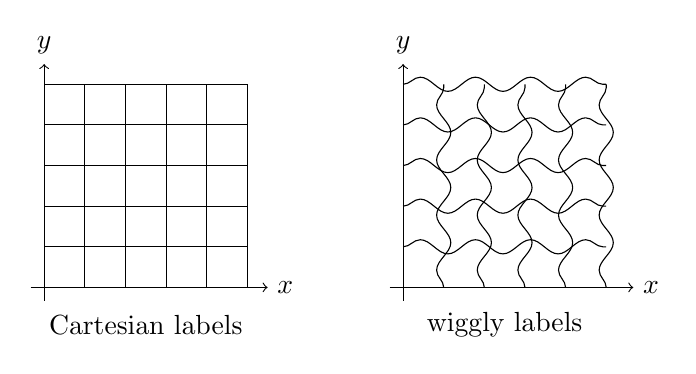
\begin{tikzpicture}[scale=0.86]
\begin{scope}
\draw[->] (-0.2,0) -- (3.3,0) node[right] {$x$};
\draw[->] (0,-0.2) -- (0,3.3) node[above] {$y$};
\foreach \u in {0.6,1.2,1.8,2.4,3.0}{
  \draw (\u,0) -- (\u,3.0);
  \draw (0,\u) -- (3.0,\u);
}
\node at (1.5,-0.55) {Cartesian labels};
\end{scope}
\begin{scope}[xshift=5.3cm]
\draw[->] (-0.2,0) -- (3.4,0) node[right] {$x$};
\draw[->] (0,-0.2) -- (0,3.3) node[above] {$y$};
\foreach \u in {0.6,1.2,1.8,2.4,3.0}{
  \draw[decorate,decoration={snake,amplitude=0.09cm,segment length=0.7cm}]
    (\u,0) -- (\u,3.0);
  \draw[decorate,decoration={snake,amplitude=0.09cm,segment length=0.7cm}]
    (0,\u) -- (3.0,\u);
}
\node at (1.5,-0.55) {wiggly labels};
\end{scope}
\end{tikzpicture}
\caption{座標格子が変化する間、幾何学は平坦なままである。計量成分だけでは、摂動が物理的かどうかを決定できない。}
\end{figure}

\section{z軸に沿って進む波}

正の\(z\)方向に進む平面波を選ぶ。その位相は
\begin{equation}
 k(z-t),
\end{equation}
と書くことができ、したがって代表的な成分は
\begin{equation}
 h_{\mu\nu}(z,t)
 =h_{\mu\nu}^{(0)}\sin k(z-t).
 \label{eq:plane-wave}
\end{equation}
の形をとる。一定の位相の面は\(z-t=\text{constant}\)を満たし、したがって伝播速度は光速である。

横波・トレースレス記述では、時間添字または\(z\)添字を含む成分は消える：
\begin{equation}
 h_{0\mu}=0,
 \qquad
 h_{z\mu}=0.
 \label{eq:tt-transverse}
\end{equation}
残るのは\(x\)-\(y\)ブロックのみである。それは対称かつトレースレスであり、
\begin{equation}
 h_{xy}=h_{yx},
 \qquad
 h_{xx}+h_{yy}=0.
 \label{eq:tt-trace}
\end{equation}

\begin{figure}[htbp]
\centering
\includegraphics[width=0.84\textwidth]{lecture_10_figure_06.png}
\caption{\(z\)に沿って進む波を、横平面の積み重ねとして表したもの。生き残る\(x\)-\(y\)振幅は\(h_{xx}+h_{yy}=0\)を満たす。}
\lectureframe{00:43:36}
\end{figure}

したがって、二つの独立なパターンが存在する。\(i,j\in\{x,y\}\)に対して、それらは
\begin{equation}
 h^{\mathrm{TT}}_{ij}(z,t)
 =
 \begin{pmatrix}
 h_+ & h_\times\\
 h_\times & -h_+
 \end{pmatrix}
 \sin k(z-t).
 \label{eq:polarization-matrix}
\end{equation}
と表示できる。対角パターンはプラス偏極と呼ばれる。非対角パターンはクロス偏極と呼ばれる。横軸を\(45^\circ\)回転させると一方のパターンが他方に変わり、任意の直線偏極波は二つの重ね合わせである。この理論にはこれ以上独立な偏極は存在しない。

\begin{figure}[htbp]
\centering
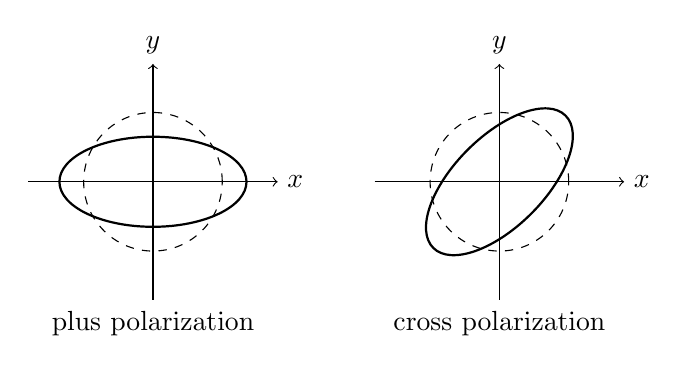
\begin{tikzpicture}[scale=0.88]
\begin{scope}
\draw[->] (-1.8,0) -- (1.8,0) node[right] {$x$};
\draw[->] (0,-1.7) -- (0,1.7) node[above] {$y$};
\draw[dashed] (0,0) circle (1.0);
\draw[thick] (0,0) ellipse (1.35 and 0.65);
\node at (0,-2.05) {plus polarization};
\end{scope}
\begin{scope}[xshift=5.0cm]
\draw[->] (-1.8,0) -- (1.8,0) node[right] {$x$};
\draw[->] (0,-1.7) -- (0,1.7) node[above] {$y$};
\draw[dashed] (0,0) circle (1.0);
\draw[thick,rotate=45] (0,0) ellipse (1.35 and 0.65);
\node at (0,-2.05) {cross polarization};
\end{scope}
\end{tikzpicture}
\caption{半周期は一つの横方向を伸ばすと同時に垂直方向を縮める。半周期後、変形は逆転する。}
\end{figure}

\section{計量成分から物理的ひずみへ}

\(z\)と\(t\)を固定し、横平面を調べる。純粋なプラス波に対して、
\begin{equation}
 ds_\perp^2
 =(1+h_{xx})\,dx^2+(1-h_{xx})\,dy^2.
 \label{eq:transverse-distance}
\end{equation}
\(h_{xx}>0\)のとき、\(x\)方向の固定された座標間隔はわずかに大きい固有長をもち、対応する\(y\)間隔はわずかに小さい固有長をもつ。半周期後、\(h_{xx}\)は符号を変え、役割は逆転する。正方形は交互に水平に伸びて垂直に縮み、次に水平に縮んで垂直に伸びる。クロス偏極に対しては、同じ交替が\(45^\circ\)回転した軸に沿って起こる。

一次の桁では、最初に長さ\(L\)であった腕は
\begin{equation}
 \frac{\Delta L}{L}\simeq\frac12 h_{ij}n^i n^j,
 \label{eq:fractional-strain}
\end{equation}
だけ変化する。ここで\(\mathbf n\)は腕に沿う方向を向く。この式は計量の摂動を、検出器が測定する無次元のひずみに翻訳する。

\begin{classroomqa}
\audiencequestion{メートル尺は電磁気的に結合されており、座標とともに単純にその静止長を変えるわけではない。むしろ、自由に離れた試験質量を用いるべきだろうか。}
\lecturerresponse{この区別は重要である。実在の棒には弾性があるため、潮汐場はその内部に応力を駆動する。鋼の棒と木の棒は一般に異なる量だけ応答する。自由に吊るされた試験質量はその特定の弾性応答を避け、相対加速度をより直接的に明らかにする。いずれの場合でも、通過する波は単に点にラベルを付け直しているだけではない。その時間依存の曲率が物理的効果を生む。
\lecturetimestamp{00:47:23--00:48:48}}
\end{classroomqa}

正確な局所的記述は測地線偏差である。\(\xi^i\)だけ離れた近傍の自由落下粒子に対して、
\begin{equation}
 \frac{d^2\xi^i}{dt^2}
 =-R^i{}_{0j0}\,\xi^j.
 \label{eq:geodesic-deviation}
\end{equation}
弱い横波・トレースレス波では、
\begin{equation}
 R_{0i0j}=-\frac12\ddot h^{\mathrm{TT}}_{ij},
 \label{eq:tidal-curvature}
\end{equation}
であるから、振動する計量は交互に潮汐加速度を生む。これが、時間依存の波を静的な物差しの選択として片付けられない理由である。それは非零の曲率を持つ。

\begin{classroomqa}
\audiencequestion{その領域のあらゆる物差しが影響を受けるなら、何が圧縮と伸長を測定できるのか。}
\lecturerresponse{ひずみゲージは、物質体に誘起された真正の応力を記録できる。さらに良いのは、自由に吊るされた質量の変化する間隔を監視することである。静的で一様な再スケーリングは測定装置に吸収できてしまうが、振動する曲率は記録可能な応答を駆動する。
\lecturetimestamp{00:51:10--00:52:02}}
\end{classroomqa}

\section{源と検出器}

電磁波は運動する電荷と電流によって生成される。重力波は運動する質量とエネルギーの分布によって生成される。エネルギーと運動量の保存により、孤立系に対する重力単極放射と双極放射は排除されるので、主要な放射モーメントは四重極である。コンパクト連星はまさに必要な変化する四重極を供給する。二つの高密度天体が互いの周りを回り、遠方場へ波を放つ。

連星に近いところでは時空は強く曲がっており、式~\eqref{eq:weak-split}の線形展開は信頼できない。遠方では、外向きの波はより大きな面積に広がり、その振幅は小さくなり、線形化された記述が正確になる。源から\(z\)軸上にいる観測者にとって、測定可能な伸縮は横方向の\(x\)-\(y\)面内にある。

\begin{classroomqa}
\audiencequestion{図中の物差しは抽象的な座標物差しなのか、物理的なメートル尺なのか。また、可変の物差しがどうやって効果を測定できるのか。}
\lecturerresponse{それは物理的物体であってもよいが、その場合にはその材料特性が重要になる。曲率が潮汐応力を供給し、鋼と木はその下で同一に変形する必要はない。それらの応答を比較すること自体がすでに測定である。より清浄な検出器は、棒を離れた試験質量に置き換え、それらの差動運動を測定する。
\lecturetimestamp{00:54:00--00:55:19}}
\end{classroomqa}

共振検出器は一つの戦略である。機械系が入射波の周波数に近い固有振動数を持つなら、波はそれをコヒーレントに駆動し、応答を増幅する。干渉計は別の戦略を用いる。鏡が試験質量の役割を果たし、レーザー干渉が垂直な腕の実効長を比較する。プラス偏光の波は一方の腕を伸ばすと同時に他方を縮める。これはまさに干渉計が検出するように設計された差動信号である。

\begin{classroomqa}
\audiencequestion{これは重力波検出器の基礎になるだろうか。}
\lecturerresponse{はい。剛い棒はほとんど変化しないが、自由に吊るされた端の質量は相対加速度を受ける。また、共振を利用して、弱い周期的駆動がより大きな応答を生むようにすることもできる。予想される天体物理的ひずみは\(10^{-21}\)の桁で極めて小さく、したがって検出器設計は、その微小な差動運動を測定可能な信号に変える技術である。
\lecturetimestamp{00:55:20--00:57:10}}
\end{classroomqa}

\begin{classroomqa}
\audiencequestion{LIGOはそのような検出器の例か。}
\lecturerresponse{はい。その基本的な観測量は、垂直な腕の中の鏡の間で反射されるレーザー光から得られる。重力波は相対的な光路長を変え、したがって干渉縞を変える。この講義の時点では、この装置はまだ直接検出を行っていなかった。その歴史的状況は後に変わった。\editorialnote{最初の直接観測であるGW150914は2015年に記録され、2016年に発表された。}
\lecturetimestamp{00:57:16--00:58:05}}
\end{classroomqa}

\begin{classroomqa}
\audiencequestion{波動解からどのような伝播速度が導かれるか。}
\lecturerresponse{光速である。位相\(k(z-t)\)は\(z\)の1単位に対して\(t\)の1単位だけ進み、線形化されたアインシュタイン方程式は電磁波方程式と同じ光円錐伝播構造をもつ。
\lecturetimestamp{00:58:07--00:58:16}}
\end{classroomqa}

ブラックホール衝突とコンパクト連星は特に有望な波源である。衝突の近傍では重力場は激しく非線形であり、解放されたエネルギーの相当な部分が重力放射として放出されうる。信号が遠方の検出器に到達するころには、その振幅は線形波動伝播が優れた記述となるほど弱くなっている。したがって重力放射は、放出された光に依存する必要のない天文学的なチャネルを開く。

\section{連星パルサーと間接的証拠}

放射はエネルギーを運ぶ。連星が重力波を放出するならば、軌道エネルギーは減少し、天体はゆっくりと内側へ螺旋を描き、軌道周期は変化する。連星パルサーはその変化を測定するのに十分精密な時計を提供する。観測された軌道進化は、一般相対性理論が予言するエネルギー損失と定量的に一致する。

講義の歴史的な文脈では、これが決定的な間接的証拠であった。地球を通過する波をまだどの検出器も捉えていなかったが、軌道は重力放射が要求する割合でエネルギーを失っていた。波は、その波源に及ぼす影響を通じてすでに観測可能であった。

\begin{classroomqa}
\audiencequestion{元の連星パルサー系を特徴づける周波数または周期は何か。それはミリ秒スケールか。}
\lecturerresponse{ミリ秒スケールとはパルサーの自転を指し、二つの星の軌道を指すのではない。教室ではその値を確認し、軌道周期が約\(7.75\)時間であることを見出す。この区別は重要である。重力放射は連星の軌道運動を追跡するが、電波パルスはそれを追跡するために用いられる精密な時計を提供する。
\lecturetimestamp{01:01:27--01:03:28}}
\end{classroomqa}

\begin{classroomqa}
\audiencequestion{数十年の観測にわたって蓄積された軌道タイミングの変化はどれほどであったか。}
\lecturerresponse{引用された蓄積されたずれはおよそ30秒である。瞬間的な相対変化はごく小さいが、数十年にわたる精密なパルスタイミングによって累積効果は可視的になる。
\lecturetimestamp{01:03:34--01:03:54}}
\end{classroomqa}

\section{時間依存性、曲率、線形性の限界}

\begin{classroomqa}
\audiencequestion{なぜ横方向の\(x\)-\(y\)面を選ぶのか。代わりに\(x\)と\(t\)を含む面を考えるとどうなるか。}
\lecturerresponse{波自体は\(z\)と\(t\)の両方に依存するが、横方向とはその空間的伝播方向に垂直な空間方向を指す。\(z\)に沿って進む波に対して、物理的な計量振幅は\(x\)-\(y\)ブロックで選ぶことができる。他の見かけの成分は存在しないか、除去可能な座標の揺らぎである。
\lecturetimestamp{01:02:22--01:03:17}}
\end{classroomqa}

\begin{classroomqa}
\audiencequestion{時間そのものが振動しているのか。}
\lecturerresponse{いいえ。波は時間の関数として振動する。固定された空間位置では、成分\(h_{ij}(z,t)\)は周期的に変化する。時間は場が依存する座標であり、この描像で交互に伸縮させられる対象ではない。
\lecturetimestamp{01:04:00--01:04:18}}
\end{classroomqa}

\begin{classroomqa}
\audiencequestion{すべての\(h_{0\mu}\)が消えるならば、時間方向を含む曲率は存在しないのか。}
\lecturerresponse{存在する。残った空間成分は時間に依存し、曲率はそれらの二階導関数を含む。したがって\(\partial_t^2h_{ij}\)のような導関数は成分\(R_{0i0j}\)を生成する。\(h_{\mu\nu}\)の時間添字成分が消えることは、時間依存の曲率が消えることを意味しない。
\lecturetimestamp{01:05:15--01:06:09}}
\end{classroomqa}

線形波動方程式が生じたのは、\(h\)が小さいと仮定されたからであり、座標の人工物が除去されたからではない。これらは二つの別個の操作である。ゲージ固定は物理的自由度を同定し、線形化は非線形相互作用を捨て去る。

\begin{classroomqa}
\audiencequestion{アインシュタイン方程式は非線形であるが、結果として得られる波動方程式は線形である。その線形性は非物理的な解を排除することによって生じるのか。}
\lecturerresponse{いいえ。それは小振幅近似によって生じる。\(h\)の二乗を含む項は捨て去られた。座標の揺らぎを除去することはどの解が物理的かを決めるが、方程式を線形にするものではない。
\lecturetimestamp{01:06:45--01:07:29}}
\end{classroomqa}

\begin{classroomqa}
\audiencequestion{線形化方程式を解いた後、厳密解と比べて誤差はどの程度ですか。}
\lecturerresponse{最初に省略される補正は\(h^2\)の程度である。もし\(h\sim10^{-1}\)ならば、それらは\(10^{-2}\)の程度であり、もし\(h\sim10^{-3}\)ならば、それらは\(10^{-6}\)の程度である。摂動計算は、仮定した小パラメータが実際に小さかったことを確認するために、常に後から検証されなければならない。
\lecturetimestamp{01:07:35--01:08:31}}
\end{classroomqa}

\begin{classroomqa}
\audiencequestion{高次の項が重要になると、波はその横波的性格を失うのですか。}
\lecturerresponse{本質的な横波的放射の性格は残るが、線形重ね合わせは成り立たない。強い波は他の波が運ぶ重力場と相互作用し、互いに変化せずに通り抜ける代わりに散乱する。
\lecturetimestamp{01:08:34--01:09:11}}
\end{classroomqa}

\begin{classroomqa}
\audiencequestion{力学的な波の速さは剛性と密度に依存する。時空にも剛性があると言える同様の意味はありますか。}
\lecturerresponse{類推としてのみである。物質媒質では、伝播は剛性を密度で割ったような組み合わせに依存する。電磁波と重力波は\(c\)で伝播するので、古い力学的な言葉ではそれらの媒質は極めて剛いと呼ぶことになる。現代物理学は時空に通常のヤング率を割り当てない。不変な事実は、場の方程式によって定まる光速での伝播である。
\lecturetimestamp{01:09:12--01:11:10}}
\end{classroomqa}

\section{第二の道筋：定常作用}

波の議論が完了したので、最後にもう一度視点を変える時間がある。定常作用の原理は、古典力学、電磁気学、場の理論、そして標準模型に共通する言語である。一般相対性理論も同じ構造に属する。

粒子の場合、作用は軌道に沿った積分である。場の場合、歴史は時空の各点に場の値\(\phi(x)\)を割り当て、作用は時空上の積分である：
\begin{equation}
 S[\phi]
 =\int d^4x\,
 \mathcal L\bigl(\phi,\partial_\mu\phi\bigr).
 \label{eq:field-action}
\end{equation}
十分に正則な\(\phi(x)\)はすべて考え得る歴史であり、十分に正則な経路がすべて考え得る粒子軌道であるのと同じであるが、ほとんどは解ではない。物理的な歴史は、固定された境界データの下での作用の定常点である：
\begin{equation}
 \delta S=0.
 \label{eq:stationary-action}
\end{equation}
場の場合、境界は経路の二つの端点を指定するだけでなく、時空領域を囲む。するとオイラー--ラグランジュ方程式が、指定された境界値の間の補間を選び出す。

アインシュタインの場の方程式は、まさにこの方法で得られる。変分は長いが、作用自体は単純である。それを書く前に、時空体積の適切な測度が必要である。

\section{なぜ行列式が体積を測るのか}

二次元で対角計量から始める：
\begin{equation}
 ds^2=g_{xx}\,dx^2+g_{yy}\,dy^2.
\end{equation}
辺\(dx\)と\(dy\)の座標長方形は、固有の辺の長さ\(\sqrt{g_{xx}}\,dx\)と\(\sqrt{g_{yy}}\,dy\)をもつので、その固有面積は
\begin{equation}
 dA
 =\sqrt{g_{xx}g_{yy}}\,dx\,dy.
\end{equation}
非対角成分\(g_{xy}\)が存在する場合、座標辺は直交する必要はない。補正された面積は
\begin{equation}
 dA
 =\sqrt{g_{xx}g_{yy}-g_{xy}^2}\,dx\,dy
 =\sqrt{\det g}\,dx\,dy.
 \label{eq:area-determinant}
\end{equation}

\begin{figure}[htbp]
\centering
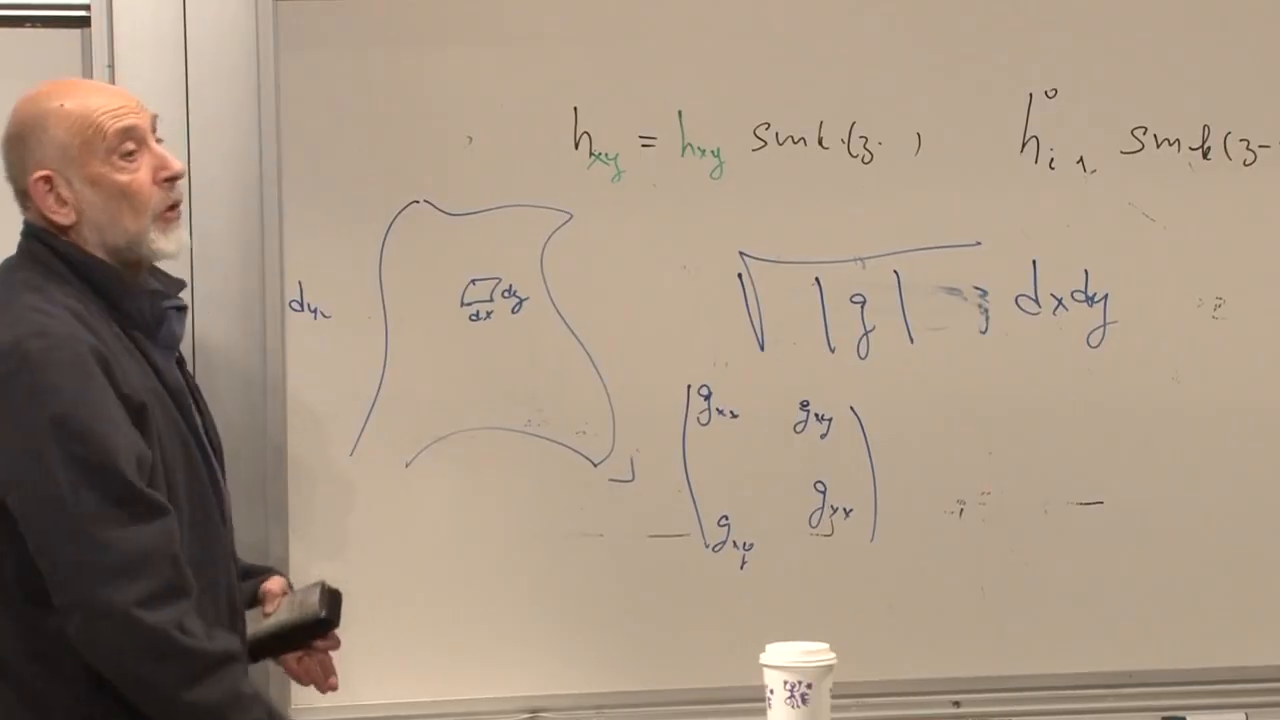
\includegraphics[width=0.84\textwidth]{lecture_10_figure_07.png}
\caption{小さな座標長方形から固有面積要素\(\sqrt{\lvert g\rvert}\,dx\,dy\)への黒板での一般化。行列式は対角の長さと非対角のずれの両方を取り込む。}
\lectureframe{01:21:25}
\end{figure}

同じ構成は任意の次元で成り立つ：
\begin{equation}
 dV_n=\sqrt{|\det g|}\,d^nx.
\end{equation}
ローレンツ時空では、もし\(g=\det(g_{\mu\nu})\)ならば、不変な四次元体積要素は慣例的に
\begin{equation}
 dV_4=\sqrt{|g|}\,d^4x,
 \label{eq:four-volume}
\end{equation}
またはmostly-plusの規約では\(\sqrt{-g}\,d^4x\)と書かれる。領域の座標は変わってもよいが、その物理的な四次元体積は変わらない。

この測度に任意のスカラー\(F(x)\)を掛けて積分すると、座標不変な量が得られる：
\begin{equation}
 \int d^4x\,\sqrt{|g|}\,F(x).
 \label{eq:invariant-scalar-integral}
\end{equation}
一般共変な理論の作用はこの形をとるべきである。そうでなければ、そこから導かれる場の方程式が座標の任意の選択に依存し得る。

\section{アインシュタイン--ヒルベルト作用}

純粋な重力では、力学場は計量そのものである。計量とその二階までの導関数から作られる最も単純な非定数スカラーはスカラー曲率\(R\)である。定数もまたスカラーであり、その係数は宇宙定数である。符号の規約と境界項を除いて、重力作用の標準的な規格化は
\begin{equation}
 S_{\mathrm{grav}}
 =
 \frac{1}{16\pi G}
 \int d^4x\,\sqrt{|g|}\,(R-2\Lambda).
 \label{eq:einstein-hilbert}
\end{equation}

\begin{figure}[htbp]
\centering
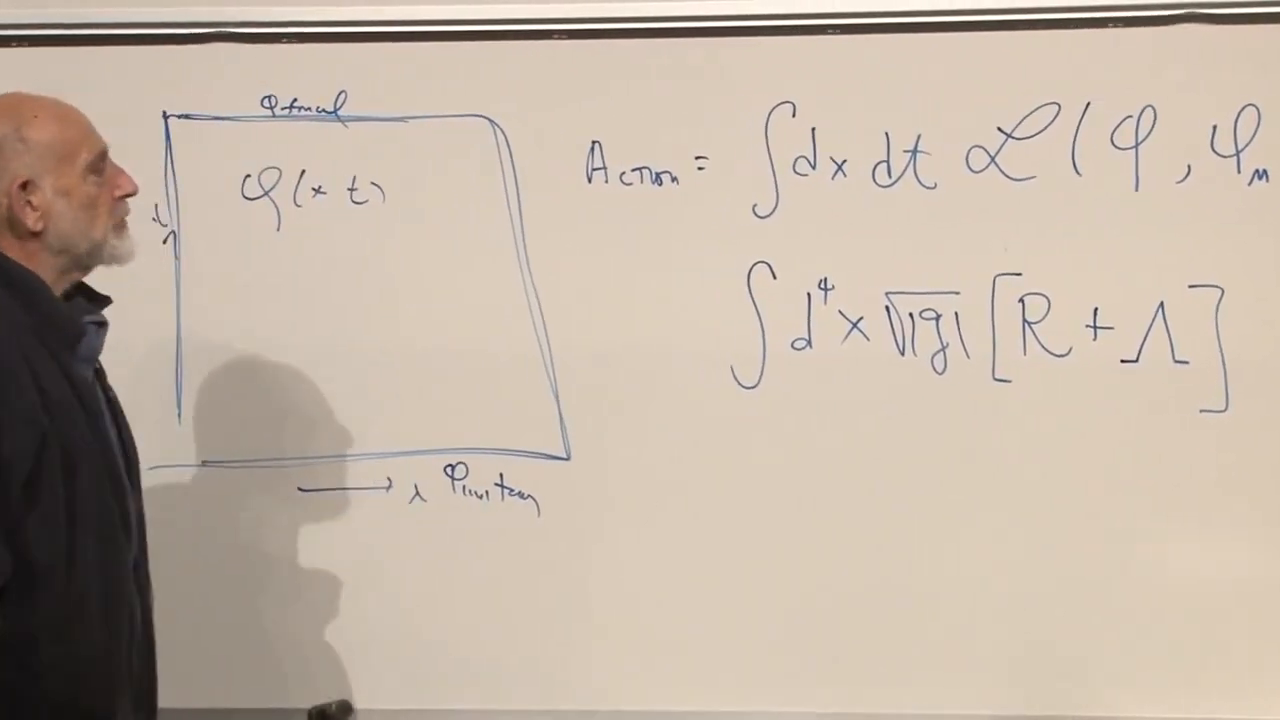
\includegraphics[width=0.84\textwidth]{lecture_10_figure_08.png}
\caption{黒板上の場の歴史の描像と重力作用。スカラー曲率が力学を与え、定数項は時空体積に比例する。}
\lectureframe{01:26:32}
\end{figure}

\(\Lambda\)に比例する項は、単に全時空体積の倍数である。以前の波動方程式は\(\Lambda=0\)の真空に対して展開されたので、そこにはその項は現れなかった。

物質は物質作用を通じて加えられる。
\begin{equation}
 S=S_{\mathrm{grav}}+S_{\mathrm{matter}}.
\end{equation}
例えば電磁気学では、不変な場の寄与は反対称テンソル\(F_{\mu\nu}\)から
構成される：
\begin{equation}
 S_{\mathrm{EM}}
 =-\frac14
 \int d^4x\,\sqrt{|g|}\,
 F_{\mu\nu}F^{\mu\nu}.
\end{equation}
全作用を逆計量に関して変分すると応力エネルギー・テンソルが定義され、
次が得られる：
\begin{equation}
 R_{\mu\nu}
 -\frac12 g_{\mu\nu}R
 +\Lambda g_{\mu\nu}
 =8\pi G\,T_{\mu\nu}.
 \label{eq:einstein-from-action}
\end{equation}
したがって、この簡潔な作用には完全な場の方程式が含まれている。真空では、
\(\Lambda=0\)として、先に調べた重力波を支配していた理論に帰着する。

\begin{classroomqa}
\audiencequestion{応力エネルギー・テンソルは作用原理のどこに入るのですか。}
\lecturerresponse{それは物質やその他の場を記述する追加項から来ます。電磁場のエネルギー、粒子場、その他のあらゆる物質的内容が\(S_{\mathrm{matter}}\)に寄与します。それらの計量変分が\(T_{\mu\nu}\)を与えます。\(\sqrt{|g|}R\)のみを含む積分が真空の重力理論です。
\lecturetimestamp{01:27:26--01:28:25}}
\end{classroomqa}

この導出は概念的には明快であり、代数的には厄介である。計量からクリストッフェル記号を構成し、曲率を構成し、縮約して\(R\)を作り、行列式因子を掛け、得られた表式を変分する。講義では、この演習は5分で終わるはずであり、失敗すれば単位を落とすことになると冗談を言い、その直後に、ずっと長い試みの末に何度も計算を放棄したことを認めている。この冗談は真剣な点を突いている。すなわち、簡潔な原理は短い成分計算を意味するとは限らない。

\begin{classroomqa}
\audiencequestion{完全な変分は相対性理論の教科書に普通に書き下されるのですか。}
\lecturerresponse{書くことはできるが、何ページにもなる。長い計算は、次のステップがなぜ続くのかを理解できる程度にまで自分で進めて初めて啓発的になる。行を次々と受動的に読むだけでは、そのような理解はほとんど得られない。現代の記号計算・数値計算ツールは帳簿付けの多くを実行できるが、それらは組織化の原理を置き換えるものではない。
\lecturetimestamp{01:31:10--01:34:16}}
\end{classroomqa}

このような計算には伝統的に二つの道がある。どのテンソルの組み合わせが可能かを見通せるほど強い幾何学的直観を養うか、代数を注意深く押し進めるかである。ほとんどの研究は両者の混合を用い、しばしば最長の縮約をコンピュータに任せる。講義では、どちらの道を選んでも生き残る原理を意図的に強調してきた。

\begin{classroomqa}
\audiencequestion{後から見れば、この作用はきわめて動機づけられたものに見える。なぜ特殊相対性理論から一般相対性理論への道はアインシュタインにとってこれほど多くの年数を要したのか、そして彼は早くから最終理論を目指していたのか。}
\lecturerresponse{必要な幾何学が知られた後では、終着点はより単純に見える。当時、必要とされた微分幾何学はほとんどの物理学者にとって馴染みのないものであり、アインシュタインは数学的な助け、とりわけマルセル・グロスマンの助けを借りてそれを学び、適応させなければならなかった。曲がった時空の概念を構築し、正しい場の方程式を見出すのにおよそ十年を要したことは、遅い達成ではなかった。初期の論文と最終的な論文は、その道中でどれほど多くを発明しなければならなかったかを示しているまさにその点で、読む価値がある。
\lecturetimestamp{01:34:20--01:35:59}}
\end{classroomqa}

したがって、この四半期は同じ理論の二つの相補的な形式で終わる。場の方程式は、曲率が応力エネルギーに局所的にどのように応答するかを語る。作用原理は、時空の全歴史が一つの不変汎関数の停留点であると述べる。弱い遠方場では、どちらの記述も、光速で実の曲率を運ぶ横波に帰着する。